\documentclass[9pt,pdftex,aspectratio=1610]{beamer}
\usepackage{amsmath, amsthm, amssymb}
\usepackage{color}
\usepackage{hyperref}
\usepackage{subfigure}
\usepackage{tabularx}
\usepackage{ragged2e}
\usepackage{booktabs}
\usepackage{multirow}
\usepackage{natbib}

\usecolortheme{dolphin}
\linespread{1.3}
\definecolor{nblue}{RGB}{0,0,128}

\bibliographystyle{ecta}
\setbeamercovered{transparent}

\newcolumntype{Y}{>{\RaggedRight\arraybackslash}X}
%\setbeamerfont{alerted text}{series=\bfseries}

\hypersetup{colorlinks=true, linkcolor=nblue,
citecolor=nblue, urlcolor=nblue, bookmarks=false,
pdfpagemode=UseNone,
pdfstartview={XYZ null null 1.25},
pdftitle={Heterogeneous Agent Trade},
pdfauthor={ Michael E. Waugh},
pdfkeywords={economics, trade, dynamics, quant econ, consumption, data science,
waugh, incomplete markets, inequality, Ricardo, julia, Armington, China, trade war, tariffs, python, matplotlib}}

%\usepackage[pdftex,colorlinks=true, bookmarks=false,
%pdfstartview={XYZ null null 1.0},
%pdftitle={Heterogeneous Agent Trade},
%pdfauthor={Michael E. Waugh},
%pdfkeywords={economics, trade, dynamics, quant econ, consumption, data science,
%waugh, incomplete markets, inequality, Ricardo, julia, Armington, China, trade war, tariffs, python, matplotlib},
%colorlinks=true,linkcolor=darkgray,citecolor=darkgray,urlcolor=darkgray,
%breaklinks]{hyperref}

\setbeamertemplate{navigation symbols}{}
\setbeamertemplate{footline}[frame number]
\setbeamertemplate{theorems}[numbered]
\setbeamertemplate{itemize subitem}[circle]
\setbeamertemplate{enumerate items}[default]

\setbeamerfont{frametitle}{size= \large}
\setbeamerfont{ framesubtitle }{size = \footnotesize}
\setbeamertemplate{frametitle}
{
\medskip
\smallskip
{\textsf{\underline{\insertframetitle\phantom{))))))))}}}}}
\setbeamertemplate{items}[circle]
\setbeamertemplate{itemize subitem}[circle]

\theoremstyle{definition}


\newtheorem{as}{Assumption}
\newtheorem{df}{Definition}
\newtheorem{lm}{Lemma}
\newtheorem{prp}{Proposition}

\usepackage[normalem]{ulem}
\newcommand\redout{\bgroup\markoverwith
{\textcolor{red}{\rule[.5ex]{1pt}{1pt}}}\ULon}

\makeatletter
\def\blfootnote{\xdef\@thefnmark{}\@footnotetext}
\makeatother

%%%%%%%%%%%%%%%%%%%%%%%%%%%%%%%%%%%%%%%%%%%%%%%%%%%%%%%%%%%%%%%%%%%%%%%%%%%%%%%%%%%%%%%%%%%%%%%%%
%%%%%%%%%%%%%%%%%%%%%%%%%%%%%%%%%%%%%%%%%%%%%%%%%%%%%%%%%%%%%%%%%%%%%%%%%%%%%%%%%%%%%%%%%%%%%%%%%

%%%%%%%%%%%%%%%%%%%%%%%%%%%%%%%%%%%%%%%%%%%%%%%%%%%%%%%%%%%%%%%%%%%%%%%%%%%%%%%%%%%%%%%%%%%%%%%%%
%%%%%%%%%%%%%%%%%%%%%%%%%%%%%%%%%%%%%%%%%%%%%%%%%%%%%%%%%%%%%%%%%%%%%%%%%%%%%%%%%%%%%%%%%%%%%%%%%

\title{\Large Heterogeneous Agent Trade}
\institute[Foo and Bar]{\normalsize\begin{tabular}[h]{c}
Michael E. Waugh  \\
Federal Reserve Bank of Minneapolis\blfootnote{The views expressed herein are those of the author and not necessarily those of the Federal
Reserve Bank of Minneapolis or the Federal Reserve System.} and NBER\\
\href{https://twitter.com/tradewartracker}{@tradewartracker}
\end{tabular}}

\date{\today}

\begin{document}

\begin{frame}
\titlepage
\setcounter{framenumber}{0}
\section{}
\end{frame}

\begin{frame}[t]{This paper\ldots}
\textbf{1.} Measure tariff-induced changes in consumption (and labor market outcomes) at a narrow geographic level.\\
\begin{itemize}
\smallskip
\item How? I proxy consumption with the universe of new auto sales in the US at monthly frequency, county level. And correlate it with policy actions in the US-China Trade War.
\smallskip
\item Clear evidence that Chinese retaliation had an impact. Both auto sales and employment $\searrow$ in high-tariff counties relative to low-tariff counties.
\end{itemize}
\bigskip
\bigskip
\textbf{2.} Use a heterogenous agent + multi-region, multi-country trade model to interpret \textbf{1.} and measure the welfare effects.
\begin{itemize}
\smallskip
\item How? Simulate and solve the model's dynamic response to tariff shocks and news about them.
\smallskip
\item Still work in progress. Today|numerical examples and demonstrate ``proof of concept.''
\end{itemize}
\end{frame}

%%%%%%%%%%%%%%%%%%%%%%%%%%%%%%%%%%%%%%%%%%%%%%%%%%%%%%%%%%%%%%%%%%%%%%%%%%%%%%%%%%%%%%%%%%%%%%%%%
%%%%%%%%%%%%%%%%%%%%%%%%%%%%%%%%%%%%%%%%%%%%%%%%%%%%%%%%%%%%%%%%%%%%%%%%%%%%%%%%%%%%%%%%%%%%%%%%%

\begin{frame}[t]{Model: Production and Trade}
\smallskip
$M$ countries. Each country produces a nationally differentiated product as in Armington.\\
\medskip
In country $i$, competitive firms' produce variety $i$ with:
\begin{align*}
Q_i = A_i N_i,
\end{align*}
where $A_i$ is TFP; $N_i$ are the efficiency units of labor supplied by households.\\
\bigskip
\medskip
Cross-country trade faces obstacles:
\begin{itemize}
\smallskip
\item iceberg trade costs $d_{nk}$ for a good to go from supplier $j$ to buyer $i$,
\end{itemize}
\bigskip
\medskip
This structure leads to the following prices consumers face
\begin{align*}
p_{ij} = \frac{d_{ij}w_{j}}{A_{j}}.
\end{align*}
\end{frame}

%%%%%%%%%%%%%%%%%%%%%%%%%%%%%%%%%%%%%%%%%%%%%%%%%%%%%%%%%%%%%%%%%%%%%%%%%%%%%%%%%%%%%%%%%%%%%%%%%
%%%%%%%%%%%%%%%%%%%%%%%%%%%%%%%%%%%%%%%%%%%%%%%%%%%%%%%%%%%%%%%%%%%%%%%%%%%%%%%%%%%%%%%%%%%%%%%%%

\begin{frame}[t]{Model: Households I}
\medskip
Mass of $L_i$ households in each country $i$.\\
\medskip
Preferences:
\begin{align*}
\small
& E_{0} \sum_{t = 0}^{\infty} \beta^{t} \tilde{u}( \{ c_{ij,t} \}_{M})\\
\\
\mbox{where}  \ \ \ & \tilde{u}( c_{ij,t} ) =  u(c_{ij,t}) + \epsilon_{j,t}.
\end{align*}
\begin{itemize}
\item $\epsilon_{j,t}$ are iid (across time and households) taste shocks over national varieties.
\end{itemize}
\medskip
Some assumptions:
\begin{itemize}
\smallskip
\item $\epsilon_{j,t}$ are distributed Type 1 Extreme Value with dispersion parameter $\sigma_{\epsilon}$.
\smallskip
\item I'll do most of the work just simply assuming $u$ is well behaved. But think CRRA if you want.
\end{itemize}
\end{frame}

%%%%%%%%%%%%%%%%%%%%%%%%%%%%%%%%%%%%%%%%%%%%%%%%%%%%%%%%%%%%%%%%%%%%%%%%%%%%%%%%%%%%%%%%%%%%%%%%%
%%%%%%%%%%%%%%%%%%%%%%%%%%%%%%%%%%%%%%%%%%%%%%%%%%%%%%%%%%%%%%%%%%%%%%%%%%%%%%%%%%%%%%%%%%%%%%%%%

\begin{frame}[t]{Model: Households II}
A household's efficiency units $z_t$ evolve according to a first-order Markov Chain. They face the wage per efficiency unit $w_{i,t}$.\\
\bigskip
Households borrow or accumulate a non-state contingent asset, $a$, with gross return $R_{i}$. Household's face the debt limit
\begin{align*}
a_{t+1} \geq - \phi_{i}
\end{align*}\\
\bigskip
Conditional on a variety choice, a household's budget constraint is
\begin{align*}
p_{ij}c_{ijt} +  a_{t+1} \leq    R_{i} a_{t} + w_{i,t} z_{t}.
\end{align*}
\end{frame}

%%%%%%%%%%%%%%%%%%%%%%%%%%%%%%%%%%%%%%%%%%%%%%%%%%%%%%%%%%%%%%%%%%%%%%%%%%%%%%%%%%%%%%%%%%%%%%%%%
%%%%%%%%%%%%%%%%%%%%%%%%%%%%%%%%%%%%%%%%%%%%%%%%%%%%%%%%%%%%%%%%%%%%%%%%%%%%%%%%%%%%%%%%%%%%%%%%%

\begin{frame}[t]{What Households Do\ldots}
Focus on a stationary setting. A household's state are it's asset holdings $a$ and shock $z$.\\
\medskip
\textbf{1.} The hh makes a variety choice (e.g. a US or Italian variety) and how much to consume of it. The choice probability (and measure of hh's consuming that variety) is:
\begin{align*}
\pi_{ij}(a, z) = \exp \left( \frac{ v_{ij}(a, z) }{\sigma_{\epsilon}} \right) \Bigg / \sum_{j'} \exp \left( \frac{ v_{ij'}(a, z) }{\sigma_{\epsilon}} \right),
\end{align*}
where $v_{ij}$ are the hh's value function conditional on a choice.\\
\bigskip
\medskip
\textbf{2.} The hh makes an asset choice. Away from the constraint, this must respect this Euler Equation:
\begin{align*}
\frac{u'(c_{ij}(a,z))}{p_{ij}} = \beta \mathrm{E}_{z'} \bigg \{ -\sigma_{\epsilon} \frac{\partial \pi_{ii}(a',z') / \pi_{ii}(a',z')}{\partial a'} + \frac{u'(c_{ii}(a',z'))R_i}{p_{ii}} \bigg \}.
\end{align*}
where I'm exploiting an ACR-like feature that value functions can be put in terms of home choices.\\
\bigskip
\textbf{Key issue: a hh's intra- and inter-temporal choices are linked.}
\end{frame}



\begin{frame}[t]{Aggregation}
Aggregates (trade, consumption, etc.) arise from explicit aggregation of hh-level actions.\\
\bigskip
To see this through trade, bilateral imports and exports are
\begin{align*}
M_{ij} = L_i \int_{z} \int_{a}  p_{ij} c_{ij}(a, z) \pi_{ij}(a, z) \lambda_i(a, z), \ \ \ \ \ X_{ji} = L_j \int_{z} \int_{a}  p_{ji} c_{ji}(a, z) \pi_{ji}(a, z) \lambda_i(a, z).
\end{align*}
where $\lambda_i$ is the distribution of households across states and $c_{ij}(a, z)$ is the consumption function.\\
\bigskip
\medskip
And one can construct the standard national income accounting identity
\begin{align*}
p_{i} Y_{i}  = \widetilde{P_{i} C_i} + \underbrace{\bigg[\ \sum_{j\neq i}X_{ji} -  \sum_{j\neq i}M_{ij} \bigg]}_{-R_{i}A_i + A_{i}'},
\end{align*} 
where trade is non-trivially connected to a county's capital account. 
\end{frame}

%%%%%%%%%%%%%%%%%%%%%%%%%%%%%%%%%%%%%%%%%%%%%%%%%%%%%%%%%%%%%%%%%%%%%%%%%%%%%%%%%%%%%%%%%%%%%%%%%
%%%%%%%%%%%%%%%%%%%%%%%%%%%%%%%%%%%%%%%%%%%%%%%%%%%%%%%%%%%%%%%%%%%%%%%%%%%%%%%%%%%%%%%%%%%%%%%%%
\begin{frame}[t]{Equilibrium}
\textbf{The Decentralized Stationary Equilibrium.} A Decentralized Stationary Equilibrium are asset policy functions and commodity choice probabilities $\{\  g_{ij}(a, z), \pi_{ij}(a, z) \ \}_{i}$, probability distributions $\{ \ \lambda_i(a, z) \ \}_{i}$ and positive real numbers $\left \{w_i, p_{ij}, R_i\right \}_{i,j}$ such that
\begin{itemize}
\smallskip
\item[i]  Prices ($w_i, p_{ij}$) satisfy the firms problem;
\item[ii] The policy functions and choice probabilities solve the household's optimization problem;
\item[iv] The probability distribution $\lambda_i(a, z)$ induced by the policy functions, choice probabilities, and primitives satisfies the law of motion and is stationary;
\item[v] Goods market clears:
\begin{align*}
p_{i} Y_{i} - \sum_{j}^{M}  X_{ji} = 0, \ \ \forall i
\end{align*}
\item[v] Bond market clears with
\begin{align*}
\mathrm{A_i'} = 0, \ \ \forall i.
\end{align*}
\end{itemize}
\end{frame}

%%%%%%%%%%%%%%%%%%%%%%%%%%%%%%%%%%%%%%%%%%%%%%%%%%%%%%%%%%%%%%%%%%%%%%%%%%%%%%%%%%%%%%%%%%%%%%%%
%%%%%%%%%%%%%%%%%%%%%%%%%%%%%%%%%%%%%%%%%%%%%%%%%%%%%%%%%%%%%%%%%%%%%%%%%%%%%%%%%%%%%%%%%%%%%%%%


\begin{frame}[t]{The H-A Trade Elasticity}
\textbf{The H-A Trade Elasticity:} The trade elasticity between country $i$ and country $j$ is:
\begin{align}
\theta_{ij} = 1 + \int_{a} \int_{z} \bigg \{ \theta_{ij}(a,z)^{I} + \theta_{ij}(a,z)^{E} \bigg \}\omega_{ij}(a,z) - \bigg \{ \theta_{ii}(a,z)^{I} + \theta_{ii}(a,z)^{E} \bigg \}\omega_{ii}(a,z), \nonumber
\end{align}
which is the difference between $ij$ and $ii$ expenditure-weighted micro-level elasticities. The micro-level elasticities for households with states $a,z$ are an intensive and extensive elasticity
\begin{align}
\nonumber
\begin{alert}<2>{\theta_{ij}(a,z)^{I} = \frac{\partial c_{ij}(a,z)/ c_{ij}(a,z)}{\partial d_{ij} / d_{ij}}}\end{alert}, \ \ \ \ \ \ \begin{alert}<3>{\theta_{ij}(a,z)^{E} = \frac{\partial \pi_{ij}(a,z) / \pi_{ij}(a,z)}{\partial d_{ij} / d_{ij}}}\end{alert}, \ \ \ \
\end{align}
and $\omega_{ij}(a,z)$ are the expenditure weights.\\
\only<2>{
\medskip
{\small \begin{align*}
\begin{alert}<2>{\theta_{ij}(a,z)^{I} = \bigg [-\frac{\partial g_{ij}(a,z)/ p_{ij}c_{ij}(a,z)}{\partial p_{ij}/ p_{ij}} - 1 \bigg ]\frac{\partial p_{ij}/p_{ij}}{\partial d_{ij}/ d_{ij}}.}\end{alert}
\end{align*}}\\
\medskip
The idea here is that reduction in trade costs relaxes the hh's budget constraint and then the division of new resources between assets and expenditure determines the intensive margin elasticity.}
\only<3>{
\medskip
{\small
\begin{align*}
\begin{alert}<3>{\theta_{ij}(a,z)^{E}}\end{alert} = - \frac{\partial \Phi_{i}(a,z) / \Phi_{i}(a,z)}{\partial d_{ij}/d_{ij}} + \begin{alert}<3>{\frac{1}{\sigma_{\epsilon}}\frac{\partial v_{ij}(a,z)}{\partial d_{ij}/d_{ij}} }\end{alert}.
\end{align*}}\\
Ignore the $\Phi_{i}(a,z)$ term. Key is \begin{alert}<3>{$\frac{\partial v_{ij}(a,z)}{\partial d_{ij}/d_{ij}}$}\end{alert}.\\
\bigskip
In the paper, I show that if relative risk aversion $ > 1$ than hh's with (i) high $u'(c)$ and (ii) high MPCs are more price elastic. \textbf{That is poor hh's are the most price sensitive.}}
\end{frame}


%%%%%%%%%%%%%%%%%%%%%%%%%%%%%%%%%%%%%%%%%%%%%%%%%%%%%%%%%%%%%%%%%%%%%%%%%%%%%%%%%%%%%%%%%%%%%%%%
%%%%%%%%%%%%%%%%%%%%%%%%%%%%%%%%%%%%%%%%%%%%%%%%%%%%%%%%%%%%%%%%%%%%%%%%%%%%%%%%%%%%%%%%%%%%%%%%


%\begin{frame}[t]{Micro-Level Elasticities}
%Intensive Margin Elasticity
%{\small \begin{align*}
%\underbrace{\frac{\partial c_{ij}(a,z)/ c_{ij}(a,z)}{\partial d_{ij} / d_{ij}}}_{\theta_{ij}(a,z)^{I}} &= \bigg [-\frac{\partial g_{ij}(a,z)/ p_{ij}c_{ij}(a,z)}{\partial p_{ij}/ p_{ij}} - 1 \bigg ]\frac{\partial p_{ij}/p_{ij}}{\partial d_{ij}/ d_{ij}}.
%\end{align*}}The idea here is that reduction in trade costs relaxes the hh's budget constraint and then the division of new resources between assets and expenditure determines the intensive margin elasticity.\\
%\bigskip
%\medskip
%Extensive Margin Elasticity
%{\small
%\begin{align*}
%\underbrace{ \frac{\partial \pi_{ij}(a,z) / \pi_{ij}(a,z)}{\partial d_{ij} / d_{ij}} }_{\theta_{ij}(a,z)^{E}} &= - \frac{\partial \Phi_{i}(a,z) / \Phi_{i}(a,z)}{\partial d_{ij}/d_{ij}} + \frac{1}{\sigma_{\epsilon}}\frac{\partial v_{ij}(a,z)}{\partial d_{ij}/d_{ij}} .
%\end{align*}}
%Ignore the $\Phi_{i}(a,z)$ term. Key issue is $\frac{\partial v_{ij}(a,z)}{\partial d_{ij}/d_{ij}}$.\\
%\medskip
%In the paper, I show that if relative risk aversion $ > 1$ than hh's with high $u'(c)$ and MPCs are more elastic. \textbf{That is poor hh's are the most price sensitive in this economy.}
%\end{frame}

%%%%%%%%%%%%%%%%%%%%%%%%%%%%%%%%%%%%%%%%%%%%%%%%%%%%%%%%%%%%%%%%%%%%%%%%%%%%%%%%%%%%%%%%%%%%%%%%
%%%%%%%%%%%%%%%%%%%%%%%%%%%%%%%%%%%%%%%%%%%%%%%%%%%%%%%%%%%%%%%%%%%%%%%%%%%%%%%%%%%%%%%%%%%%%%%%


\begin{frame}[t]{Trade Elasticities by HH-Level State}
\vspace{-.5cm}
\begin{figure}[t]
\centerline{
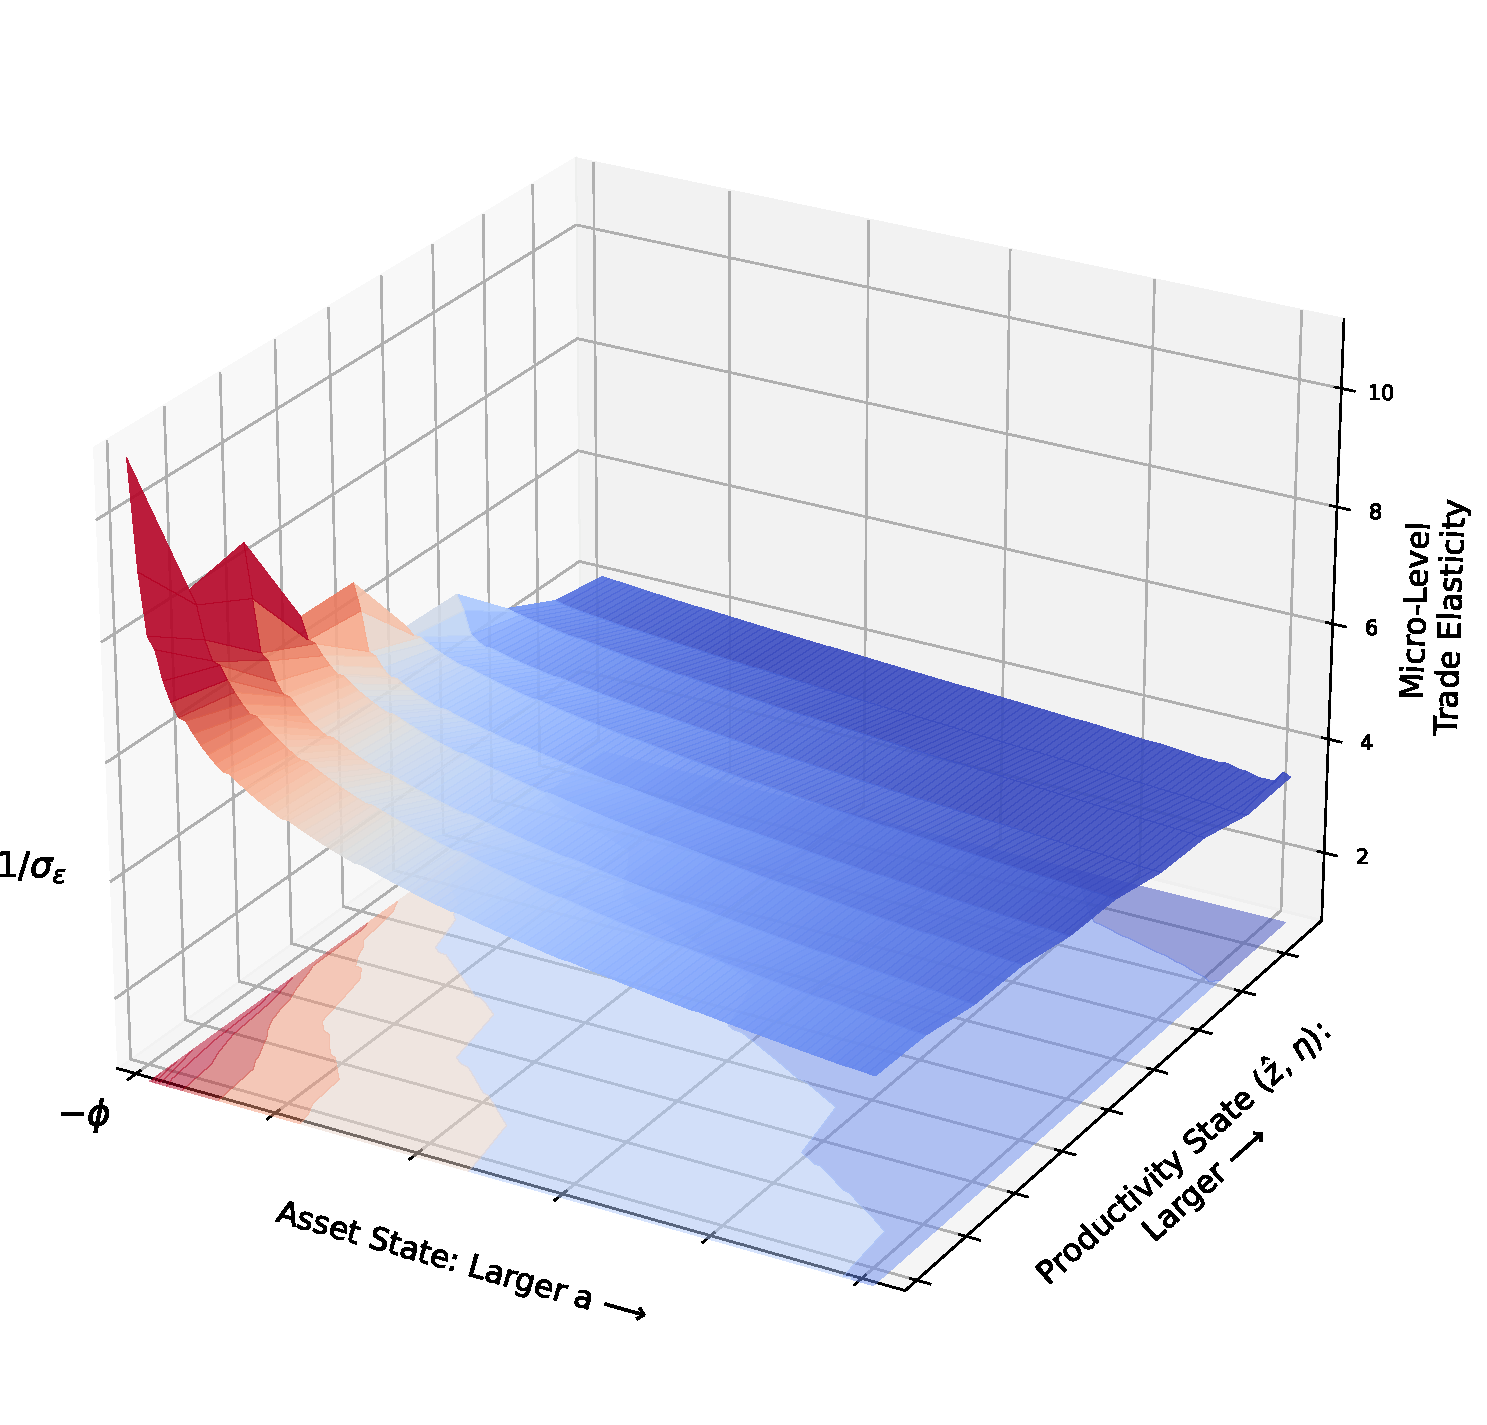
\includegraphics[scale = 0.5]{../notes/figures/micro-elasticity.pdf}}
\end{figure}
\end{frame}


\begin{frame}[t]{Trade Shares: $M_{ij}(a,z) / M_{ii}(a,z)$, by HH-Level State}
\vspace{-.5cm}
\begin{figure}[t]
\centerline{
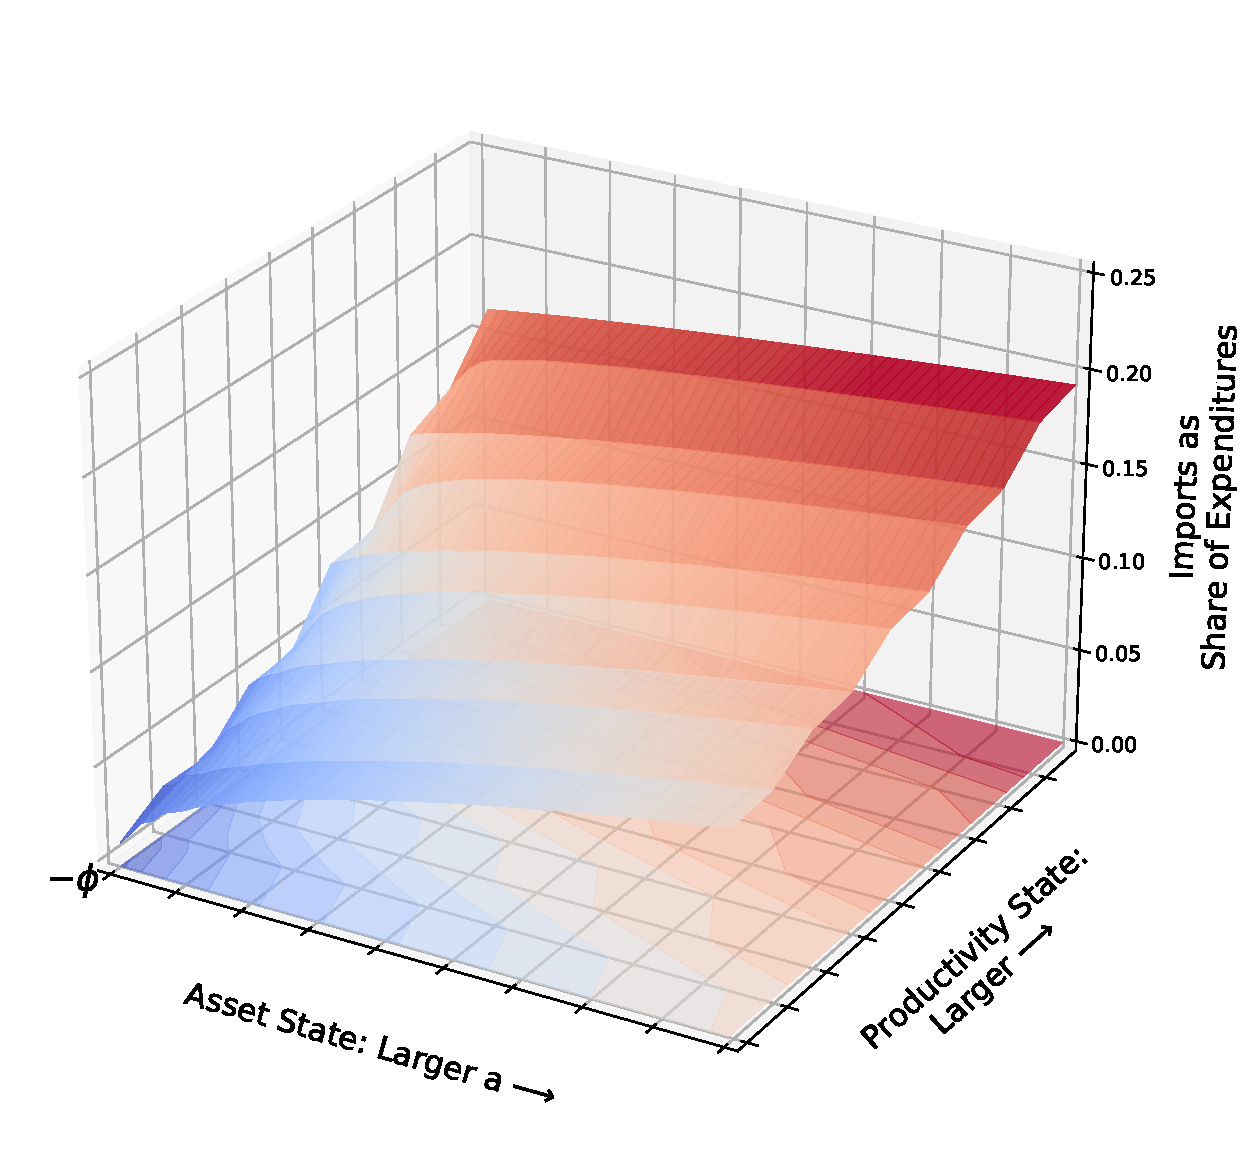
\includegraphics[scale = 0.5]{../notes/figures/trade-share.pdf}}
\end{figure}
\end{frame}


\begin{frame}[t]{H-A Gains from Trade}
\textbf{H-A Welfare Gains from Trade:} The gains from trade under a utilitarian social welfare function are
\begin{align*}
\frac{\mathrm{d} W_{i}}{\mathrm{d} d_{ij} / d_{ij}} = \int_{z} \int_{a}  \bigg \{ \underbrace{\frac{\mathrm{d} v_i(a, z)}{\mathrm{d} d_{ij} / d_{ij}}}_{\small \mbox{gains to hh}}  + \underbrace{v_{i}(a,z) \frac{\mathrm{d} \lambda_{i}(a,z)/ \lambda_{i}(a,z)}{\mathrm{d} d_{ij} / d_{ij}}}_{\small \mbox{gains to reallocation}}   \bigg \} L_i \lambda_{i}(a,z).
\nonumber
\end{align*}
where $v_i$ is a hh's value function before taste shocks are realized.\\
\medskip
Household-level gains are
\begin{align*}
\frac{\partial v_i(a, z)}{\partial d_{ij} / d_{ij}} = \mathbb{E}_{z} \sum_{t = 0}^{\infty} \beta^{t} \bigg \{ -\sigma_{\epsilon} \frac{\mathrm{d} \pi_{ii}(a_{t},z_{t}) / \pi_{ii}(a_{t},z_{t})}{\mathrm{d}d_{ij} / d_{ij}} + u'(c_{ii}(a_{t},z_{t}))a_{t} \times \frac{\mathrm{d} R_{i}}{\mathrm{d} d_{ij} / d_{ij}} \bigg \}
\end{align*}\\
\bigskip
The gains to a hh pick up two effects:
\begin{itemize}
\item An ACR-like term reflecting how it's home choice changes\ldots basically the gains from substitution.
\smallskip
\item How the value of a hh's wealth changes through GE effects on interest rates. 
\end{itemize}
\end{frame}

%%%%%%%%%%%%%%%%%%%%%%%%%%%%%%%%%%%%%%%%%%%%%%%%%%%%%%%%%%%%%%%%%%%%%%%%%%%%%%%%%%%%%%%%%%%%%%%%
%%%%%%%%%%%%%%%%%%%%%%%%%%%%%%%%%%%%%%%%%%%%%%%%%%%%%%%%%%%%%%%%%%%%%%%%%%%%%%%%%%%%%%%%%%%%%%%%

\begin{frame}[t]{H-A Gains from Trade: $\log$ Preferences $\Rightarrow$ Separation of Trade and H-A}
\textbf{Separation of Trade and Micro-Heterogeneity:} In the dynamic, heterogenous agent trade model where preferences are logarithmic over the physical commodity
\begin{align}
\tilde{u}( c_{ij,t} ) =  \log(c_{ij,t}) + \epsilon_{j,t}, \nonumber
\end{align}
the trade elasticity is
\begin{align}
\theta = -\frac{1}{\sigma_{\epsilon}}, \nonumber
\end{align}
and is independent of household heterogeneity.\\
\medskip
And the welfare gains from trade are
\begin{align}
\frac{\mathrm{d} W_{i}}{\mathrm{d} d_{ij} / d_{ij}} = -\frac{1}{\theta (1-\beta)} \times \frac{\mathrm{d} \pi_{ii} / \pi_{ii}}{\mathrm{d}d_{ij} / d_{ij}}. \nonumber
\end{align}
and is (i) independent of the household heterogeneity and (ii) summarized by the trade elasticity and the change in the home choice probability (and home share).
\end{frame}

%%%%%%%%%%%%%%%%%%%%%%%%%%%%%%%%%%%%%%%%%%%%%%%%%%%%%%%%%%%%%%%%%%%%%%%%%%%%%%%%%%%%%%%%%%%%%%%%
%%%%%%%%%%%%%%%%%%%%%%%%%%%%%%%%%%%%%%%%%%%%%%%%%%%%%%%%%%%%%%%%%%%%%%%%%%%%%%%%%%%%%%%%%%%%%%%%

\begin{frame}[t]{H-A Gains from Trade under Efficiency}
\textbf{Trade Elasticities and Welfare Gains in the Efficient Allocation} The elasticity of trade to a change in trade costs between $i,j$ in the efficient allocation is:
\begin{align}
\theta_{ij} =  -\frac{1}{\sigma_{\epsilon}} \bigg [ u'(c_{ij}) c_{ij} \bigg]. \nonumber
\end{align}\\
\bigskip
And the welfare gains from a reduction in trade costs between $i,j$ are
\begin{align}
\frac{\mathrm{d} W}{\mathrm{d} d_{ij} / d_{ij}} = \frac{\partial W}{\partial d_{ij} / d_{ij}} = \frac{1}{1-\beta} \times u'(c_{ij}) c_{ij} \pi_{ij} L_i, \nonumber
\end{align}
which is the discounted, direct effect from relaxing the resource constraint.
\end{frame}

%%%%%%%%%%%%%%%%%%%%%%%%%%%%%%%%%%%%%%%%%%%%%%%%%%%%%%%%%%%%%%%%%%%%%%%%%%%%%%%%%%%%%%%%%%%%%%%%
%%%%%%%%%%%%%%%%%%%%%%%%%%%%%%%%%%%%%%%%%%%%%%%%%%%%%%%%%%%%%%%%%%%%%%%%%%%%%%%%%%%%%%%%%%%%%%%%

\begin{frame}[t]
\frametitle{My Progress Report}
\textbf{What I've done:}
\begin{itemize}
\item Measured tariff-induced changes in consumption at a narrow geographic level: auto sales growth fell by $\approx$ 4 p.p. in high-tariff counties relative to low-tariff counties.
\smallskip
\item Evidence that the fall in consumption relates to a reduction in production and labor market opportunities for those most exposed.
\smallskip
\item As of now, all this is $\approx$ consistent with what comes out of a forward-looking/ dynamic heterogenous agent +  multi-region, multi-country trade model.
\end{itemize}
\bigskip
\textbf{I'm working on now!}
\begin{itemize}
\item A real calibration/ estimation of model and welfare analysis. Improved treatment of asset market. Talk to me in a month.
\smallskip
\item My RA Thomas Hasenzagl and I are piecing together a public GITHUB repository with code to implement Heterogenous Agent Trade (HAT) models, fast and efficiently.
\end{itemize}
\end{frame}

%%%%%%%%%%%%%%%%%%%%%%%%%%%%%%%%%%%%%%%%%%%%%%%%%%%%%%%%%%%%%%%%%%%%%%%%%%%%%%%%%%%%%%%%%%%%%%%%
%%%%%%%%%%%%%%%%%%%%%%%%%%%%%%%%%%%%%%%%%%%%%%%%%%%%%%%%%%%%%%%%%%%%%%%%%%%%%%%%%%%%%%%%%%%%%%%%

\appendix

\newcounter{finalframe}
\setcounter{finalframe}{\value{framenumber}}

\begin{frame}[allowframebreaks]
\frametitle{References}
\scriptsize
\bibliography{../notes/bibtex/micro_price_bibtex}
\end{frame}


%%%%%%%%%%%%%%%%%%%%%%%%%%%%%%%%%%%%%%%%%%%%%%%%%%%%%%%%%%%%%%%%%%%%%%%%%%%%%%%%%%%%%%%%%%%%%%%%%
%%%%%%%%%%%%%%%%%%%%%%%%%%%%%%%%%%%%%%%%%%%%%%%%%%%%%%%%%%%%%%%%%%%%%%%%%%%%%%%%%%%%%%%%%%%%%%%%%







\setcounter{framenumber}{\value{finalframe}}

%%%%%%%%%%%%%%%%%%%%%%%%%%%%%%%%%%%%%%%%%%%%%%%%%%%%%%%%%%%%%%%%%%%%%%%%%%%%%%%%%%%%%%%%%%%%%%%%%
%%%%%%%%%%%%%%%%%%%%%%%%%%%%%%%%%%%%%%%%%%%%%%%%%%%%%%%%%%%%%%%%%%%%%%%%%%%%%%%%%%%%%%%%%%%%%%%%%



\end{document} 